\documentclass[12pt]{article}
\usepackage{graphics}
\begin{document}
\newcounter{problem}
\thispagestyle{empty}

\section*{random extra problems}

\paragraph{Problem~\theproblem}\refstepcounter{problem}%
Consider a slab of air with density $\rho$ of height $\Delta y$ and
perpendicular (that is, horizontal) area $A$, with volume $A\,\Delta
y$.  If this air is in equilibrium with its surroundings, it neither
rises nor falls, so its weight is supported by a pressure difference
$\Delta P$.

\textsl{(a)}~Draw a free-body diagram for the slab and find an
expression for the pressure difference $\Delta P$ in terms of $\Delta
y$ and whatever else you need.

\textsl{(b)}~In the ideal gas law, there is a relationship between
$P$, $V$, $N$, and $T$.  Convert this into a relationship between $P$
and $\rho$.  \emph{Hint:} Recall that $\rho$ is a mass per unit
volume; you might need to use the average mass of an air molecule.

\textsl{(c)}~Rearrange your result from part (a) using your result
from part (b) to get a differential equation that relates
$\mathrm{d}\rho/\mathrm{d}y$ to $\rho$.  Integrate this equation to
get the density $\rho$ as a function of $y$ for the atmosphere,
assuming that it is \emph{isothermal} (it isn't).

\textsl{(d)}~Comment on the relationship between your answer and the
Boltzmann factor discussed in your textbook.

\paragraph{Problem~\theproblem}\refstepcounter{problem}%
In practice problem 14.58, you will show that in one period of
oscillation, a weakly damped harmonic oscillator loses energy $\Delta
E = 2\pi\,E/Q$, where $E$ is the mechanical energy in the oscillator
and $Q$ is the quality factor, defined to be the ratio
$Q\equiv\omega_0/\gamma$.  If this oscillator is driven by a driving
force so that instead of decaying, its amplitude is held constant, how
much average mechanical power does the driving force have to supply to
the oscillator?  A typical mechanical clock has a pendulum with a mass
of 2~kg, a period of 1~s, and a quality factor of 20.  What is the
power in W required to keep this pendulum swinging at an amplitude of
4~cm?

\paragraph{Problem~\theproblem}\refstepcounter{problem}%
Consider a one-dimensional wave on a string of the form
\begin{equation}
y = y_0 \cos(k\,x + \omega\,t)
\end{equation}
with $y_0= 1.0\times 10^{-2}~\mathrm{m}$, $k= 1.0~\mathrm{m^{-1}}$,
and $\omega= 2.0~\mathrm{s^{-1}}$.  What is the velocity $\vec{v}$
(speed and direction) of the wave?  Draw three quantitative diagrams
showing (a)~the displacement $y$ as a function of time $t$ for a fixed
point at $x= +1.047~\mathrm{m}$, (b)~the displacement $y$ as a
function of position $x$ for a fixed time $t=0$, and (c)~the
displacement $y$ as a function of position $x$ for a fixed time $t=
1.047~\mathrm{s}$.

\paragraph{Problem~\theproblem}\refstepcounter{problem}%
Two wave pulses, labeled A and B, are approaching each other on a rope
as shown.  The rope has mass per unit length $\mu= 0.1~{\rm
kg\,m^{-1}}$ and is held under constant tension $T= 10~{\rm N}$.
Recall that although the waves travel in the $+x$ and $-x$ directions,
each piece of the rope is only moving in the $y$ direction.
\\ \rule{0.1\textwidth}{0pt}
\resizebox{0.8\textwidth}{!}{\includegraphics{../pro/twopulse.eps}}

(a) What is the wave speed $c$ in the rope?

(b) Draw a graph of the instantaneous $y$-direction speed $v_y$ of the
rope as a function of $x$ for the instant shown above.  Be
quantitative; carefully label all interesting positions and speeds.
Also, pay attention to the {\em sign} (positive or negative) of the
speed.

(c) On your graph, point out the locations where the rope feels a $y$
component of force and indicate the sign (positive or negative) of the
force at each location.

\paragraph{Problem~\theproblem}\refstepcounter{problem}%
A continuation of Problem 3: Draw a graph of the rope configuration
at the time at which the two wave pulses are exactly coincident.  In
what form is the ``energy'' of the wave pulses at this moment?

\paragraph{Problem~\theproblem}\refstepcounter{problem}%
In a mechanical watch, the oscillator is a metal wheel with moment of
inertia $I$ attached to a torsional spring.  Model the torsional
spring as making a restoring torque $\tau$ which is proportional to
its angular displacement $\theta$ from its equilibrium orientation by
the equation
\begin{equation}
\tau = -\kappa\,\theta \nonumber
\end{equation}
Derive the differential equation relating $\theta$ to its second
derivative (with respect to time).  What is the period $T$ of
oscillation?  As the watch gets warmer, the metal wheel expands.  If
it expands (in radius) by a factor of $1.0001$ (ie, $1+10^{-4}$), does
the period go up or down?  If the watch originally kept perfect time,
how many seconds per day does it gain or lose after the expansion?
Assume (incorrectly) that the torsional spring is unaffected by the
thermal expansion.

\end{document}
